% CREATED BY DAVID FRISK, 2018

% IMPORT SETTINGS
\documentclass[12pt,a4paper]{article}
\usepackage[utf8]{inputenc}
\usepackage{float}

\setlength{\parindent}{0pt}
\setlength{\parskip}{\baselineskip}
\usepackage[a4paper, margin=1in]{geometry}

\usepackage[noconfigs, swedish]{babel}
\usepackage{hyperref}
\hypersetup{breaklinks=true}

\usepackage{titling}
\newcommand{\subtitle}[1]{%
  \posttitle{%
    \par\end{center}
    \begin{center}\large#1\end{center}
    \vskip0.5em}%
}

\usepackage{graphicx}

\begin{document}

\pagenumbering{gobble}

\title{Learn You a Physics for Great Good}
\subtitle{Using domain specific languages to teach physics}
\date{\today}
\author{Björn Werner\\ Erik Sjöström \\ Johan Johansson \\ Oskar Lundström}

\maketitle

% TABLE OF CONTENTS
\newpage
\tableofcontents

% START OF MAIN DOCUMENT
\newpage
\setcounter{page}{1}
\pagenumbering{arabic}			% Arabic numbering starting from 1 (one)
%\setlength{\parskip}{0pt plus 1pt}

\section{Bakgrund}

% Varför
På civilingenjörsprogrammet Datateknik på Chalmers ingår fysikkursen
\textit{Fysik för ingenjörer}. Tentastatistiken för denna kurs är inte
jättebra\cite{tentastatistik}. Vi
tror att många studenter på datateknik, (``datateknologer''), finner denna kurs
svår eller ointressant, och att detta leder till att ungefär en
tredjedel av kursdeltagarna får underkänt på tentamen.

Examinatorn för kursen ``Fysik för ingenjörer, TIF085 (2016)'' Åke Fäldt, tycker
att studenter i allmänhet verkar ha svårt för att sätta upp egna
modeller. De baserar sina mentala modeller helt eller delvis på
intuition och felaktiga antaganden, istället för definitioner och
bevisade satser som man är säker på gäller. Detta leder till att de
tar genvägar som ofta är fel.

%TODO: PaJa: använd inte "DSL" som förkortning för kursen - det kan orsaka förvirring med begreppet DSL i allämnhet. Skriv DSLM eller DSLsofMath. [Här och på fera ställen nedan.]
Sedan våren 2016 har kursen ``Domain Specific Languages of
Mathematics'' (``DSL'') eller ``Matematikens domänspecifika språk'' givits som en
valbar kurs på kandidatnivå för studenter på Chalmers och Göteborgs Universitet. År
2016 var Cezar Ionescu huvudföreläsare, och från 2017 är Patrik
Jansson huvudföreläsare. Det direkta målet är att förbättra den
matematiska utbildningen för
datavetare och den datavetenskapliga utbildningen för
matematiker, och den grundläggande idéen bakom kursen är att ``uppmuntra studenterna
att närma sig matematiska domäner från ett funktionellt
programmeringsperspektiv: att ge beräkningsbevis (calculational
proofs); att vara uppmärksamma på syntaxen för matematiska uttryck;
och, slutligen, att organisera de resulterande funktionerna och
typerna i domänspecifika
språk.''.\cite{lecture-notes}\cite{tfpie2015}
Konkret så presenterar kursen matematik så som derivator, komplexa
tal och matriser ur ett funktionellt programmeringsperspektiv i
Haskell. Dessa för studenterna bekanta verktyg används för att lösa
matematiska problem så som modellering av syntax, evaluering till
semantiska värden, och datorassisterad bevisföring.

Även på MIT har en kurs inte helt olik DSL tidigare givits som berör både fysik
och DSL. ``Classical Mechanics: A Computational Approach'' gavs av
Prof Geral Sussman och Prof. Jack Wisdom bl.a. år
2008.\cite{classical-mechanics-course-mit-2008}
Denna kurs på avancerad nivå studerar de fundamentala principerna av klassisk mekanik
med hjälp av beräkningsidéer för att precist formulera principerna av
mekanik, med början i Lagranges ekvationer och avslut i
perturbationsteori. I kursen används boken ``Structure and
Interpretation of Classical Mechanics'' av Sussman, Wisdom, och Mayer,
vilken förklarar fysikaliska fenomen genoma att visa datorprogram för att
simulera dem, skrivna i språket Scheme.\cite{SICM}

Utöver DSL-kursen har det även tidigare gjorts ett kandidatarbete om DSL
här på Chalmers. År 2016 på vårterminen utfördes kandidatarbetet
``Programmering som undervisningsverktyg för Transformer, signaler och
system. Utvecklingen av läromaterialet TSS med DSL'' av fem studenter
från Datateknik och Teknisk Matematik på Chalmers. Arbetet bestod av
utveckling av läromaterial med tillhörande programmeringskod,
uppgifter, och lösningar, som komplement till existerande kurser i
signallära.\cite{kandidat2016}

Vår tanke med detta kandidatarbete är att, likt premissen bakom DSL-kursen
och kandidatarbetet från 2016, med hjälp av ett bekant verktyg
som Haskell angripa fysik på ett sådant sätt att ämnet blir både
intressant och roligt för datateknologer, och därmed förhoppningvis
också enklare. Med hjälp av domänspecifika språk skrivna i Haskell för att
modellera fysik, i.e. samma pedagogiska verktyg som används inom
datakurser, tror vi att kopplingen mellan fysikkursen och
datateknikprogrammet kan göras tydligare och lärandet kan underlättas.
Förhoppningen är att bl.a. det kraftfulla typsystemet i Haskell ska
hjälpa studenter att bygga mentala modeller som är korrekta och inte
bygger på felaktiga intuitioner.

% Relevant för
Projektet är relevant för datateknologer som läser en fysikkurs. Men
det kan också bli relevant för en fysikstudent som är ute efter en
inkörsport till funktionell programmering. Förhoppningsvis blir det
också relevant för de som är intresserade av domänspecifika språk i
stort, pedagoger och föreläsare inom de berörda områdena och kanske
till och med programledningen som ser vår rapport som ett skäl att
introducera innehåll av detta slag i till exempel fysikkursen.

För läsaren som inte är insatt i domänspecifika språk, kan det
förklaras som ett språk konstruerat för ett specifikt område, en
domän. Språket kan användas för att enklare uttrycka saker inom
domänen, till exempel Newtons andra lag $F=m \cdot a$ än vad som är
möjligt inom generella (programmerings)språk. För vidare läsning
rekommenderas \textit{DSL for the Uninitiated}.\cite{DSLU}


% \subsection{Vad?}
%
% Vi vill med detta projekt skapa ett pedagogiskt läromaterial som med hjälp av en eller flera DSL:er ska fungera som ett komplement till de kurser i fysik som riktar sig till studenter inom datateknik.
%
% \subsection{Relevant för?}
%
% Förhoppningsvis blir det också relevant för de som är intresserade av DSL:er i stort, pedagoger och föreläsare inom de berörda områdena
% %
% %PaJa: angående "skifta läroplanen" - det är oklart vad ni menar här. Formulera om med tanke på rubriken "relevant för" - programledning kanske vill utveckla / förbättra programmet, etc.
% och kanske till och med programledningen som ser vår rapport som ett skäl att skifta läroplanen.
%
% \subsection{Relaterat till?}
%
% %PaJa: bra med referenser - men gör en .bib-fil och citera ordentligt.
% Detta arbete kan relateras det arbete som redan utförts inom detta område t.ex. \textit{Structure and Implementation of Classical Mechanics}\cite{SICM}.
% %PaJa: citera mer specifikt (kursen, artikeln, eller båda). [Det är heller inte specifikt bara "analys".]
% Och även det arbete som Patrik Jansson utfört med att brygga gapet inom analys.
% %PaJa: OK, men bör kanske formuleras om för att tydliggöra.
% Vi skulle också gärna se att vårt arbete kan relateras till den större diskussionen om varför matte och fysik lärs ut inom data.
%

\section{Syfte}

Syftet med projektet är att skapa domänspecifika språk för fysik samt ett tillhörande läromaterial. Läromaterialet ska både förklara fysik och parallellerna med de domänspecifika språken. Förhoppningen är att väcka intresse för fysik hos datateknologer genom att presentera fysik från ett annat perspektiv.

%Syftet är en kort beskrivning av uppdraget och vilket resultat som uppdraget
%ska leda till.
%Projektets syfte är att implementera ett antal DSLs i ett par olika discipliner, samt
%en dokumentation över användningen av dom.
%
%\begin{itemize}
%    \item 1-2 meningar
%    \item Vad ska resultatet vara?
%\end{itemize}

\section{Problem/Uppgift}

%Oskar: Detta är min bild. Rätta om jag fått något om bakfoten
Slutprodudukten är tänkt att bli ett läromaterial som med hjälp av domänspecfika språk förklarar koncept inom fysiken. Läromaterialet ska vara en brödtext varvat med programkod och exempel skrivet på en lättsam stil, i likhet med \textit{Learn You a Haskell}\cite{LYAH} som är ett läromaterial för Haskell. Vår tanke är att presentera fysik parallellt med att vi bygger upp domänspecika språk för fysik. Vi kommer även i texten presentera fysikaliska problem och visa hur man kan modellera och lösa dem i de domänspecifika språk vi skapat tillsammans.


De uppgifter vi har framför oss är därmed:

\begin{itemize}
	\item Hitta de områden inom \textit{Fysik för ingenjörer} som datateknologer har svårt för.
	\item Inläsning av \dots
	\begin{itemize}
		\item \dots fysik.
		\item \dots domänspecifika språk.
		\item \dots liknande projekt för att få inspiration.
	\end{itemize}
	\item Skriva läromaterial och parallellt implementera egna domänspecifika språk.
\end{itemize}


Frågor som vi vill besvara när projektet är klart:
%TODO: Vissa frågor kanske ska tas bort eller omforumerlas nu när vi bytt fokus
\begin{itemize}
    \item Kan man skapa domänspecifika språk för fysik?
    \item Hur brett/djupt kan vi komma med våra domänspecfika språk?
    \item Kan man använda våra domänspecika språk för att lära ut?
    \item Kan vi skapa ett läromaterial utifrån våra domänspecifika språk?
%TODO: PaJa: notera att de två sista frågorna kräver en mer empirisk insats för att besvara. Kan kvarstå, men kanske bör synas mer i planen i så fall.
    \item Kommer vår läromaterial främja lärandet?
    \item Är djup eller ytlig inbäddning bäst ur ett pedagogiskt syfte?
\end{itemize}

\section{Avgränsningar}

Projektet kommer enbart behandla den fysik som ingår i kursen \textit{Fysik för ingenjörer}. Denna avgränsningen valdes dels för att det är så mycket fysik gruppmedlemmarna kan, dels för att det är den kursen detta projekt kan bli mest relevant för.

%TODO: PaJa: Jag tror att det i praktiken är en hel del tillämpad matematik inbäddat i kursen också, och det kan vara värt att nämna.
\textit{Fysik för ingenjörer} behandlar grunderna inom de tre områdena mekanik (inklusive stelkroppsmekanik), termodynamik och vågrörelselära. Vi har valt att i första hand prioritera mekanik, för att senare i mån av tid även behandla termodynamik och vågrörelselära. Dessutom kommer de områden datateknologer haft svårt för prioriteras. Även om projekets direkta syfte inte är att förbättra tentastatistiken på \textit{Fysik för ingenjörer}, är vår förhoppning att förståelsen för de svåra delarna ska bli bättre.

%TODO: Koppla till etik!


% Under avgränsningar talar man om vad man inte behandlar.
% Projekter avgränsar sig till exempelvis att implementera DSLs för samtliga områden
% inom kursen Fysik för ingengörer.

% \begin{itemize}
%     \item Vilka delar av det övergripande syftet som ej ska med
% \end{itemize}

\section{Metod/Genomförande}

%TODO: Gäller detta fortfarande?
Som ett genomgående tema vill vi arbeta in återkoppling med Åke och Patrik så att vi vet att vi håller oss på banan och inte gör det för svårt för oss själva eller potentiella studenter.

Den övergripande planen är att börja med att läsa in oss på fysik, domänspecika språk och liknande projekt. Detta för att få en grundläggande uppfattning av hur projeket kan tänkas se ut. Därefter kommer läromaterialet att skrivas. Eftersom domänspecifika språk kommer presenteras varvat i läromaterialet kommer därför också de domänspecika språken skapas parallellt med skrivandet. Vi vet ännu inte hur vi bra kan fördela arbetet mellan gruppmedlemmarna. En möjlighet, beroende på tidsbehovet, är att en/två skriver om mekanik och en/två om termodynamik eller våglära. Under skrivandets gång kommer en del inläsning behöva göras parallellt. Det kan handla både om fysik och domänspecika språk, till exempel att jämföra vår implementation med likaratade implementationer, för att se att vi håller oss på banan.

För att hitta de områden datateknologer har problem med i \textit{Fysik för ingenjörer} kommer vi prata med kursens föreläsare, med DNS (Datateknologsektionen på Chalmers) samt reflektera över de delar vi själva tyckte var svåra.

De primära källorna till inläsning av fysik kommer att vara kursboken \textit{University Physics}\cite{UP} samt föreläsarens egna material i form av anteckningar och övningsuppgifter. Till vår hjälp för att förstå hur man på ett bra sätt kan skapa domänspecika språk inom fysik har vi boken \textit{Structure and Interpretaton of Classical Mechanics}\cite{SICM}.

Se bilaga $\lambda$ för en mer detaljerad lista över hur vi tänkt lägga upp arbetet.

% Metodkapitlet ska beskriva hur man avser att lägga upp arbetet. Detta
% omfattar bland annat arbetsgång, design av experiment och användning av olika
% datainsamlingsmetoder. Ett metodkapitel ska, i idealfallet, vara så utförligt att
% vem som helst som har vissa baskunskaper inom området ska kunna utföra arbetet
% på det sättet som har beskrivits i rapporten och nå samma resultat. Att beskriva
% metoden är viktigt för att uppdragsgivaren ska kunna bedöma om man kan nå målet
% på det föreskrivna sättet. Det är därför också viktigt att man förklarar varför den
% valda metoden ger ett tillförlitligt resultat.

%TODO: PaJa: strukturen på dokumentet ser lite konstig ut när har en "subsection" som heter "Avslutning"
\subsection{Avslutning}

För att avsluta vårt projekt vill vi återkoppla med studenter inom data som både har läst fysikkursen och de som inte har läst den för att på så sätt få deras perspektiv på det hela. Detta skulle även ge en fingervisning om hurvida vårt resultat är tillförlitligt. Lämpliga frågor är då:

\begin{itemize}
    %\item Tror du att detta \textbf{hade} hjälpt dig när du studerade fysik?
    %\item Tror du att detta \textbf{kommer} att hjälpa dig när du studerar fysik?
    \item Tror du att detta hade gett dig ett annat perspektiv när du studerade fysik?
    \item Tror du att detta kommer att underlätta för dig när du studerar fysik?
    \item Hade det här hjälpt till att väcka intresset hos dig när du studerade fysik?
    \item Ser det roligt ut?
    \item Har vi missat nåt?
    \item Vad hade vi kunnat göra bättre?
\end{itemize}

I mån av tid så vill vi använda denna återkoppling för att förfina vårt läromaterial. Med den större förhoppningen att vi kan producera ett läromaterial som är bra nog för att publiceras.

\section{Samhälleliga och etiska aspekter}

En positiv etisk aspekt på projektet är att vi valt att prioritera de områden som varit svåra för datateknologer. Det ger med andra ord ett potentiellt nyttovärde för datateknologer som läser \textit{Fysik för ingenjörer}.

En negativ etisk aspekt är att nyttovärdet enbart gynnar de som är bra på Haskell och funktionell programmering. För att kunna tillgodogöra sig den eventuella kunskapsvinning från detta projeket krävs det att man är bra på Haskell eftersom allting uttrycks i det programmeringsspråket.

I likhet med de flesta kunskapsinsamlande projeket, även om något så ''oskyldigt'' som matematik och grundläggande fysik, uppkommer frågan om i vilka syften kunskapen kan användas. Det läromaterial vi skriver är i sig inte farligt eller missgynnande för någon. Däremot kan det användas av andra i illvilliga syften. Detta är något man behöver vara medveten om, även om det inte är något som påverkar det dagliga arbetet.

%TODO: PaJa: lite tunt. Kanske värt att skriva något om öppen källkod, öppen dokumentation? Eller något om hur korrekt förståelse av fysik kan rädda liv (genom att undvika olyckor)?




% ----------gamla nedan
%
% Nedan följer svar på de samhälleliga och etiska frågor som ställts i anvisningarna till projektplanen-
%
% 1) Vilka etiska  aspekter (värden) är relevanta för projektet?
% \[
% \emptyset
% \]
%
% Vi tycker inte det finns några negativa eller positiva etiska konsekvenser av detta projekt. Vi ska konstruera ett läromaterial om grundläggande fysik och har svårt att se hur det kan påverka någon individ eller grupp negativt.
%
% 2) Hur kan vi genomföra vårt projekt för att undvika etiska problem med vår metod?
%
% Vi kommer att kommunicera med vår handledare, en föreläsare och studenter som testar vårt material. Givet att vi är allmänt trevliga ser vi inga etiska problem med denna metod.
%
% 3) Vad kan det finnas för nytta eller etiska problem med det sannolika resultatet (utfallet) av projektet som man bör ta hänsyn till?
%
% Främjandet av fysikinlärning för datastudenter kan möjligtvis leda till positiva aspekter för samhället i stort, om inte annat för att utbildning blir lättare att ta till sig. Förhoppningsvis kan vi också göra smärre nytta för forskningen inom detta område (DSL för pedagogik?).
%
% De enda dilemman där de etiska aspekterna skulle kunna äventyras skulle antagligen vara om vårt läromedel utnyttjades för att lära ut kärnfysik till studenter i länder med kärnvapenprogram \url{http://sverigesradio.se/sida/artikel.aspx?programid=3182&artikel=2980763}.
   % Detta lär inte vara något vi behöver beakta i vårt läromedel, då kursen fysik för ingenjörer inte innefattar någon kärnfysik.
%
% 4)  Vilka berörs av projektets genomförande eller av det sannolika resultatet (utfallet) av projektet? Hur berörs de? Finns det etiska problem kopplat till detta som man bör ta hänsyn till?
%
% Se ovanstående svar.

\section{Tidsplan}

Projekets milstolpar finns nedan. Datumet anger då milstolpen bör vara avklarad.

\textbf{Milstolpar}

\begin{itemize}
    \item 2018-02-06 - Innehåll och medlemmar bestämt till halvtidsredovisning
    \item 2018-02-09 - \textbf{Planeringsrapport färdig och inlämnad}
    \item 2018-02-16 - Manus och presentationsmaterial till halvtidsredovisning skapat
    \item 2018-02-19 - Avslutat övergripande inläsning
    \item 2018-02-19 - Identifierat områden/moment som vi ska behandla
    \item 2018-02-23 - Genrepat halvtidsredovisning
    \item 2018-02-27 - \textbf{Halvtidsredovisning}
%TODO: PaJa: typo? 2018-02-03 är före alla andra milstolpar
    \item 2018-02-03 - \textbf{Egen utvärdering på blankett till handledaren}
    \item 2018-03-23 - \textbf{Bestämma rapportspråk (sv/en)}
    \item 2018-04-17 - Skrivit klart läromaterialet
    \item 2018-05-01 - Första utkast till rapport
    \item 2018-05-08 - \textbf{Inlämning av poster för tryckning}
    \item 2018-05-14 - \textbf{Slutrapport färdig och inlämnad}
    \item 2018-05-15 - \textbf{Utställning}
    \item 2018-05-15 - Skrivit klart slutredovisningen
    \item 2018-05-16 - \textbf{Engelsk titel angiven}
    \item 2018-05-21 - \textbf{Inlämning opposition}
    \item 2018-05-20 - Genrep av slutredovisning
    \item 2018-05-22 - \textbf{Slutredovisning. Eller 23 maj}
    \item 2018-05-25 - \textbf{Egen utvärdering på blankett till handledaren}
    \item 2018-06-01 - \textbf{Slutgiltig inlämning av rapport}
\end{itemize}

\textbf{Gantt-schema}

Datumet anger deadline för aktiviteten.

\begin{figure}[H]
  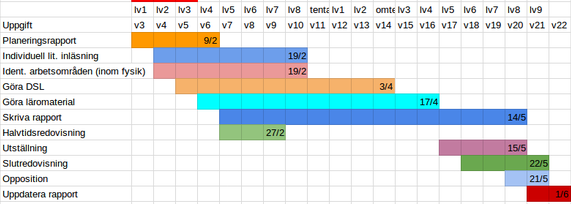
\includegraphics[width=\linewidth]{gantt.png}
  \caption{Gantt-schema.}
  \label{fig:gantt}
\end{figure}

\newpage
\pagenumbering{gobble}

%TODO: PaJa: titta igenom referenser.bib och se till att "ord" som bör ha stora bokstäver skyddas med klamrar: TSS := {TSS}, DSL := {DSL}, Haskell := {Haskell}, etc.
\bibliography{referenser}
\addcontentsline{toc}{section}{Referenser}
\bibliographystyle{ieeetr}

\newpage
\section*{Bilagor}
\label{sec:bilaga}
\addcontentsline{toc}{section}{\nameref{sec:bilaga}}

\subsection*{Bilaga $\lambda$: Detaljerad lista över metod}

\subsubsection*{Inläsning}

\begin{itemize}
    \item Identifikation av problemområden.
        \begin{itemize}
            \item Kontakt med Åke och DNS. Studera kursutvärderingar.
            \item Reflektera över vad vi själva tyckt varit svåra områden då vi läst kursen.
%TODO: PaJa: formulera om
            \item Se om Patrik har något kul att säga...
        \end{itemize}
    \item Studerande av existerande läromaterial, både inom ren fysik och liknande vårt material.
        \begin{itemize}
            \item Fysikboken.
            \item Åkes egna material.
            \item Boken \textit{Structure Interpretaton of Classical Mechanics}\cite{SICM}.
            \item Kursboken till kursen \textit{Matematikens domänspecifika språk}.
        \end{itemize}
    \item Existerande implementationer.
        \begin{itemize}
            \item OpenTA.
            \item Hamilton.
            \item MasteringPhysics.
%TODO: PaJa: formulera om
            \item Fråga om Patrik kan något mer...
        \end{itemize}
    \item Tidigare forskning.
        \begin{itemize}
            \item Cezar och Patriks 2015 paper.
            \item 2016 års kandidatarbete.
            \item Artikeln \textit{DSL for the Uninitiated}.
            \item \textit{Communicating Mathematics: Useful Ideas from Computer Science}
        \end{itemize}
\end{itemize}

\subsubsection*{Implementation av domänspecifika språk}

Vid implementationen av ett/flera domänspecika språk behöver nedanstående punkter genomföras.

\begin{itemize}
    \item Hitta relevanta grundtyper inom fysik, exempelvis sträcka och massa.
    \item Hitta relevanta komposittyper, exempelvis hastighet och tryck.
    \item Utförligt typsystem.
    \item Dimensionskontroll.
    \item Modellera fysikens syntax i språket.
    \item Pedagogiska syntaxträd.
    \item Kombinatorer och konstruktorer.
    \item Hålla våra typer polymorfa.
\end{itemize}

\subsubsection*{Skrivande av läromaterial}

Vid skrivandet av läromaterialet kommer följande punkter ligga till grund.

\begin{itemize}
    \item Frågetecken: Gemensam vokabulär (som funkar när man pratar om både fysik och programmering, generics kontra polymorfism). Och som gör det möjligt att prata om dem i samma mening utan att byta språk och på så sätt brygga det semantiska gapet mellan områdena.
    \item Övningar
        \begin{itemize}
            \item Modellera ett fysikaliskt problem med vårt domänspecifika språk.
            \item Lös ett ''vanligt'' fysikaliskt problem med hjälp av vårt domänspecifika språk.
            \item Simuleringar i stil med \textit{Bouncing Balls}.
            \item Delar av fysiken vi inte behandlat lämnas som övning att själv implementera.
        \end{itemize}
    \item Gå igenom allmän teori (t.ex. Newtons lagar, krafter som verkar, etc) tillsammans med en parallell utveckling av ett domänspecifikt språk.
    \item Materialet ska vara enkelt att ta till sig.
    \item Verkligen exponera det DSL som vi gemensamt bygger för att påvisa kopplingen mellan fysik och programmering.
\end{itemize}

\end{document}
